%----------------------------------------------------------------------------------------
%	SECTION 1.1
%----------------------------------------------------------------------------------------

\section{Discrete Random Vectors.}
\label{section1}

\begin{definition}
    Let $X=(X_1, \dots, X_n)$ be a discrete random vector, with probability
    $p(x)=P(X_1=x_1. \dots, X_n=x_n)$. We define the \textbf{entropy} of $X$ in base
     $b$ to be:
     \begin{equation}
         H_b(X) = \sum_x{p(x)\log_b{\inv{p(x)}}}
     \end{equation}
\end{definition}
\begin{remark}
    We can similarly extend the previous definitions to discrete random
    vectors.
\end{remark}

Now, consider the random vector $U=(U_1, \dots, U_k)$. We describe a
communications model where $U$ is taken to  $X=(X_1, \dots, X_k)$ via an
encoder. $X$ is then sent through a (possibly noisy) channel as the output $Y$,
which is a (possibly) noisy version of $X$. We then take  $Y$ to  $V$ through a
decoder and send  $V$ to the destination. Ideally, we want  $U=V$, however,
since $Y$ is the reesult of sending $X$ through a (possibly) noisy channel, it
may not be the case. In fact, we see that the sequence $U \rightarrow X
\rightarrow Y \rightarrow V$ forms a Markov chain.

\begin{figure}[h]
    \centering
    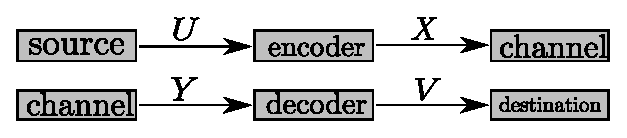
\includegraphics[scale=0.5]{Figures/Chapter2/channel.eps}
    \caption{The Sequence $U \rightarrow X \rightarrow Y \rightarrow V$ seen as
    sending $U$ to a recpient.}
    \label{fig_2.7}
\end{figure}

Now, this implies that $p(y|x)=p(v,y,x)=p(v|y)$. Notice also that $I(U,V) \leq
I(X,V) \leq I(X,Y)$. We then come to a central theorem called the \ita{data
processing theorem}.

\begin{theorem}[The Data Processing Theorem]\label{2.2.1}
    Given a Markov chain of discrete random vectors $U \rightarrow X \rightarrow
    Y \rightarrow V$, we have:
    \begin{equation}
        I(X,Y) \leq I(X,Y)
    \end{equation}
\end{theorem}

\begin{theorem}\label{2.2.2}
    If $X=(X_1, \dots, X_n)$ is a random vector, with $X_i$ and  $X_j$
    independent for each $i \neq j$, then:
    \begin{equation}
        I(X,Y) \geq \sum_{i=1}^n{I(X_i,Y_i)}
    \end{equation}
\end{theorem}
\begin{proof}
    We have:
    \begin{equation*}
        I(X,Y)=E(\log{\frac{p(x|y)}{p(x)}})=E(\log{\frac{p(x|y)}{p(x_1) \dots
        p(x_n)}})
    \end{equation*}
    On the other hand:
    \begin{equation*}
        \sum{I(X_i,Y_i)}=\sum{E(\log{\frac{p(x_i|y_i)}{p(x_i)}})}=
        E(\log{\frac{p(x_1|y_1) \dots p(x_n|y_n)}{p(x_1) \dots p(x_n)}})
    \end{equation*}
    So, by Jensen's inequality, we get:
    \begin{equation*}
        \sum{I(X_i,Y_i)}-I(X,Y) \leq \log{E(\frac{p(x_1|y_1) \dots
        p(x_n|y_n)}{p(x|y)})}=0
    \end{equation*}
\end{proof}

\begin{example}
    LEt $X_1, \dots, X_n$ be independent identically distributed random
    variables with common entropy $H$.Let $\pi$ be a permutation on the set
    $\{1, \dots, n\}$ and let $Y_i=X_{\pi(i)}$. Then $I(X,Y)=nH$, but
    $\sum{I(X_i,Y_i)}=kH$ with $k$ the number of fixed points ($\pi(x)=x$) of
    $\pi$. If  $\pi(i) \equiv i+1 \mod{n}$, then $k=0$.
\end{example}

\begin{theorem}\label{2.2.3}
    If $X=(X_1, \dots, X_n)$, and $Y=(Y_1, \dots, Y_n)$ are random vectors over
    a discrete memoryless channel, then $I(X,Y) \leq \sum{I(X_i,Y_i)}$.
\end{theorem}
\begin{corollary}
    $H(X) \leq \sum{H(X_i)}$
\end{corollary}

\begin{example}
    Let $X$ be a random variable with entropy  $H$ and let
    $X_1=\dots=X_n=Y_1=\dots=Y_n=X$. Then $I(X,Y)=H$ and $\sum{I(X_i,Y_i)}=nH$.
\end{example}
